% psyplot chapter

\part{New Software Tools for Paleoclimate Analysis}  \label{part:software}

\Chapter{Psyplot}{A flexible framework for interactive data analysis}

\label{chp:psyplot}

\begin{refsection}

%----------------------------------------------------------------------------------------
%	SECTION 1
%----------------------------------------------------------------------------------------

\section{Summary}  \label{sec:psyplot-joss}

\blockquote{
	\textit{From}
	\bibforkey{Sommer2017}
}

\noindent psyplot \citep{Sommer2017} is a cross-platform open source python project that mainly combines the plotting utilities of matplotlib \citep{Hunter2007} and the data management of the xarray \citep{HoyerHamman2017} package and integrates them into a software that can be used via command-line and via a GUI.

The main purpose is to have a framework that allows a fast, attractive, flexible, easily applicable, easily reproducible and especially an interactive visualization of data.
 
The ultimate goal is to help scientists in their daily work by providing a flexible visualization tool that can be enhanced by their own visualization scripts.

The framework is extended by multiple plugins: psy-simple \citep{Sommer2017b} for simple visualization tasks, psy-maps \citep{Sommer2017c} for georeferenced data visualization and psy-reg \citep{Sommer2017d} for the visualization of fits. It is furthermore extended by the optional graphical user interface psyplot-gui \citep{Sommer2017e}.


\section{Introduction}  \label{sec:psyplot-review}

\todo[inline, size=\normalsize]{Write visualizations review \citep{NockeSterzelBoettingerEtAl2008, RautenhausBoettingerSiemenEtAl2018, SullivanTrainorGuitton2019, SullivanKaszynski2019, BoettingerRoeber2019}}

The mathematical and statistical processing of climate data works closely together with its visualization and analysis and are usually treated in separate manners. \cite{KeimAndrienkoFeketeEtAl2008} for example, (following \cite{Wijk2005}) distinguish two steps of visual analytics, the initial data processing with statistical or mathematical techniques, and a \textit{sense-making loop} of visualization, exploration and the gain of new knowledge. \cite{BoettingerRoeber2019} distinguish the \textit{filtering} step (data processing), and \textit{mapping}/\textit{rendering} step that describes the visualization. Also in the literature there is a clear division between the climate visualization (or visual analytic) papers and the standard statistical or climate literature that describes new methods for data processing. Visualization research focuses mainly on advanced visualization tools such as ParaView \citep{Ayachit2015}, VAPOR \citep{ClyneMininniNortonEtAl2007} or Avizo\addref \citep[e.g.][]{RautenhausBoettingerSiemenEtAl2018, NockeBuschmannDongesEtAl2015, WongShenLeungEtAl2014, BoettingerRoeber2019} whereas statistical or climate literature commonly uses R \citep{RCT2019}, Python \citep{Oliphant2006, PerezGrangerHunter2011}, \glspl{cdo} \citep{Schulzweida2019} or other command-line tools.

However, these two aspects commonly interplay and the new knowledge from the visualization step will raise the need for more statistical and mathematical processing of the initial data. This calls for integrated and flexible tools that tackle both steps: the data processing and the visualization. An example for such a tool is provided through the Earth System Model Evaluation Tool (ESMValTool) \citep{EyringRighiLauerEtAl2016} that provides common diagnostics for \glspl{esm} to enable model intercomparisons. The tool, however has limited interactivity and a slow learning curve for the implementation of new diagnostics.

This lack leads to large efforts of climate scientists to develop scripts for the data processing and visualization. They usually do not follow a systematic framework and as such need to be adapted every time a new project starts and they are difficult to share with other researchers. The new \textit{psyplot} framework wants to generalize this data processing and visualization by providing a framework that is highly flexible, interoperates with standard computational data processing tools and enables flexible visualizations and adaptations. The software is written in the programming language Python \citep{PerezGrangerHunter2011} and builds upon the visualization package \textit{matplotlib} \citep{Hunter2007} and the N-dimensional array processing package \textit{xarray} \citep{HoyerHamman2017}, that closely interoperates with the numeric packages numpy and scipy \citep{JonesOliphantPetersonEtAl2001, Oliphant2006} and the parallel computing library dask \citep{DDT2016}. Due to the flexibility of Python, it can be used from the command-line, a \gls{gui} (section \ref{sec:psyplot-gui}) or jupyter notebooks\footnote{\url{https://jupyter.org/}} \citep{KluyverRaganKelleyPerezEtAl2016}. As such, it supports out-of-core computation (i.e. the processing of data too large to fit into memory), a rich set of visualization methods from matplotlib, and can be extended to other visualization packages, such as the 3D-visualization framework VTK \citep{Sommer2019a}.

The next section \ref{sec:psyplot-framework} provide an overview of the framework with it's data model, plugins and \gls{gui}, and section \ref{sec:psyplot-conclusions} discusses further usage and extensions to the software. For further information, usage and implementation examples I also refer to the online documentation\footnote{the psyplot documentation is hosted at \url{https://psyplot.readthedocs.io}}.

\section{The psyplot framework}  \label{sec:psyplot-framework}

The psyplot framework consists of three parts: The core structure that is built upon \textit{xarray} and provides the general infrastructure (section \ref{sec:psyplot-model}), the plugins that use the plotting functionalities of \textit{matplotlib} (section \ref{sec:psyplot-plugins}), and the \gls{gui} (section \ref{sec:psyplot-gui}).


\subsection{Data model}  \label{sec:psyplot-model}

\subsubsection{Psyplot and xarray}  \label{sec:psyplot-dependencies}

psyplot acts as a high-level interface into the packages \textit{xarray} and \textit{matplotlib}. The first one is a recent package for N-dimensional labeled arrays that adopts Unidata’s self-describing Common Data Model on which the network Common Data Form (netCDF) is built \citep{RewDavis1990, BrownFolkGoucherEtAl1993, HoyerHamman2017}. The package integrates with standard python from the python environment, such as the computing and analysis packages numpy \citep{Oliphant2006}, scipy \citep{JonesOliphantPetersonEtAl2001, Oliphant2007}, pandas \citep{McKinney2010} and statsmodels \citep{SeaboldPerktold2010}, but also offers intuitive interfaces for other packages, such as a package for empirical orthogonal functions \citep[EOFs, ][]{Dawson2016}, \glspl{cdo} \citep{Mueller2019}, fourier transforms \citep{UchidaRokemNicholasEtAl2019} any many more\footnote{\label{foot:xraccessors} several packages related to xarray are listed in the docs at \url{http://xarray.pydata.org/en/stable/related-projects.html} and psyplots integration (accessors) in particular is shown at \url{https://psyplot.readthedocs.io/en/latest/accessors.html}.}. This large range of extensibility distinguishes psyplot from other high-level visualization software, such as ParaView or Vapor, and they can all be implemented as a formatoption (see below) or used in a pre-processing step.

\subsubsection{Psyplot core structure}  \label{sec:psyplot-core}  

\begin{figure}
	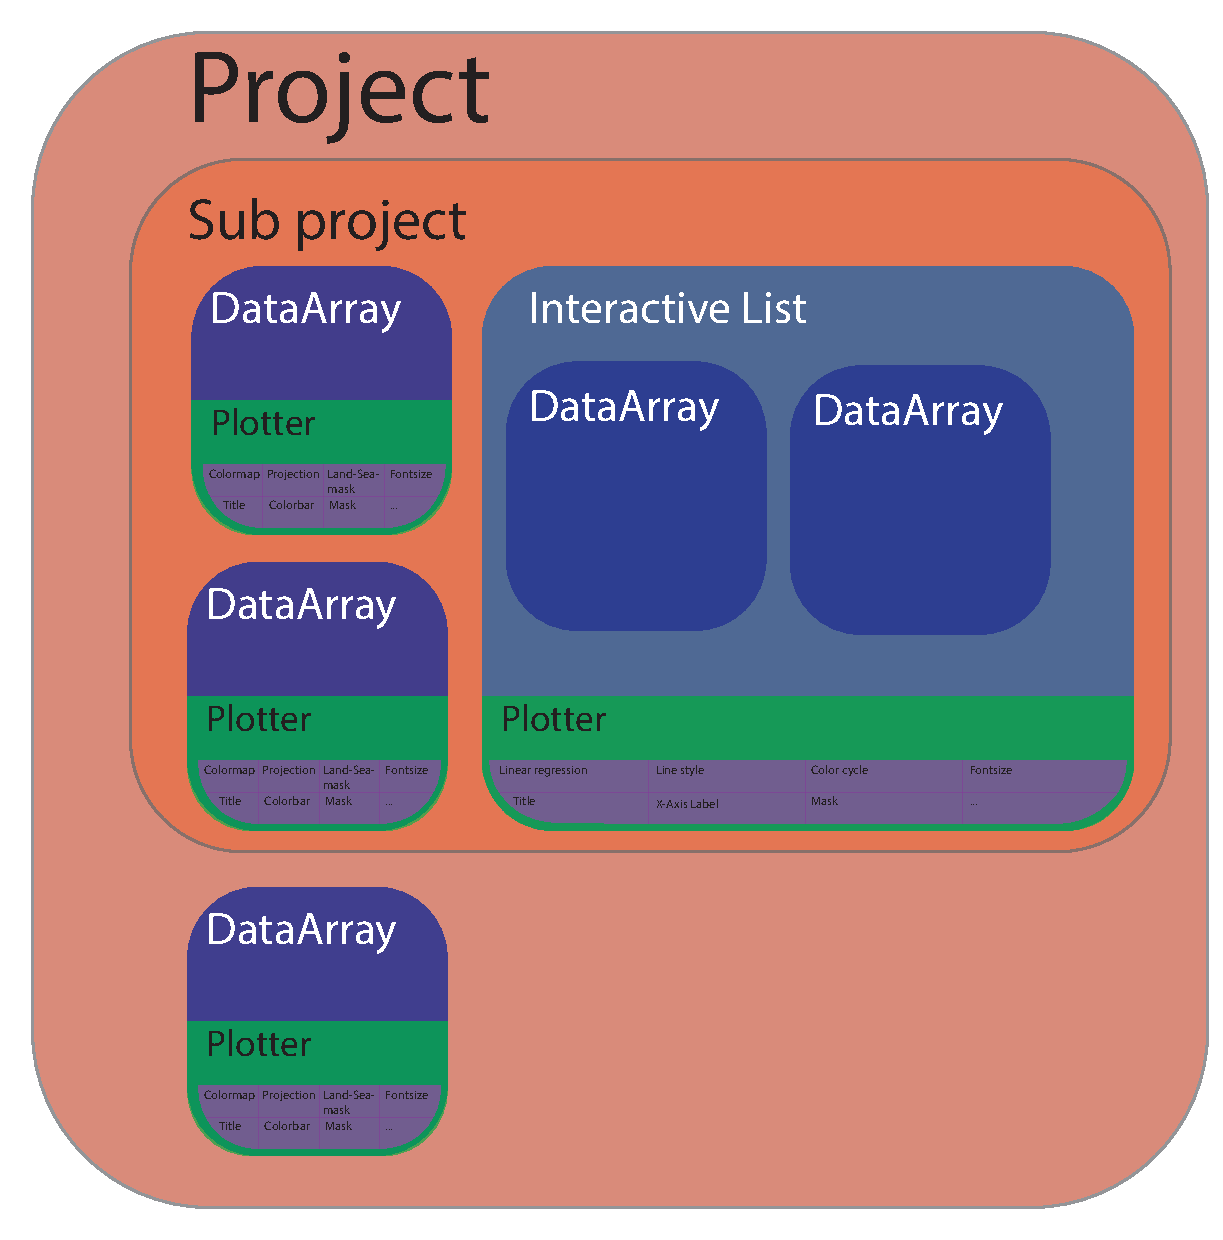
\includegraphics[width=\linewidth]{psyplot-figures/psyplot_framework.pdf}
	\caption[The psyplot core framework]{The psyplot core framework. A (sub) project consists of n-dimensional data arrays or a list of these that are each visualized by a plotter. Each plotter consists of a set of formatoptions that control the appearance of the plot or performs data manipulation.}
	\label{fig:psyplot-core}
\end{figure}

The core structure of psyplot consists of five base classes that interact with each other, the visualization objects \textit{Plotter} and its \textit{Formatoptions}, the data objects \textit{DataArray} and an \textit{InteractiveList} of them, and a collection of all of them, the psyplot \textit{Project}. It is schematically visualized in figure \ref{fig:psyplot-core}.

The most highl-evel \gls{api} object is the psyplot project that consists of multiple data objects that are (or are not) visualized. The main purpose is a parallel handling of multiple plots/arrays that may also interact with each other (e.g. through the sharing of formatoptions). It mainly spreads update commands to it's contained objects, but also serves as a filter for the data objects. Furthermore, one project may be split up into sub projects which then only control a specific part of the main project, e.g. for a specific formatting of only a small part of the data.

The next level is the \textit{DataArray} from the xarray package (or more explicitly, it's accessor, the \textit{InteractiveArray}$^{\ref{foot:xraccessors}}$), that holds the data of one (or more) variables (e.g. temperature) and its corresponding coordinates (e.g. time, latitude, longitude, etc.). It may be one or multidimensional depending on the chosen visualization method. psyplot offers several methods to provide the coordinates for the plotting of different grids to make the visualization easier. The software can interprete CF Conventions\footnote{\url{http://cfconventions.org}} and UGRID conventions for unstructured grids \citep{JagersStuebeGrossEtAl2018}.

Multiple of these arrays can also be grouped together into an \textit{InteractiveList} that shall be visualized by the same plot method (e.g. multiple lines or a scalar field with overlying vector field).

The visualization part in the framework is managed by the \textit{Plotter} class, a collection of multiple \textit{Formatoptions}. Each plotter subclass is designed to visualize the data in a specific manner (e.g. via line plots, violin plots, or map plots) and is completely defined through it’s formatoptions.

\textit{Formatoptions} are the core of the psyplot structure. The standard functionality of a formatoption is to control the visual appearance of one aspect of the plot (e.g. through the colormap, figure title, etc.). It is, however, completely unlimited and can also do data manipulations or calculations. The psy-reg plugin for example (see section \ref{sec:psyplot-plugins}) implements a formatoption that performs a regression through the data that is then visualized. As mentioned earlier, each plotter is set up through it’s formatoptions where each formatoption has a unique formatoption key inside the plotter. This formatoption key (e.g. \textit{title} or \textit{cmap}) is what is used for updating the plot, manipulating the data, etc.. Formatoptions might also interact with other formatoptions inside the plotter or from other plotters. This concept of formatoptions allows to use the same formatoption with all different kinds of plotters and the interaction of multiple plots with each other. Common plot features, such as the figure title, colormap, etc., therefore don't have to be implemented explicitly for every plotter but can be used from existing implementations. This framework also allows a very easy integration and development of own formatoptions with a low or high level of complexity.

\subsection{Psyplot plugins}  \label{sec:psyplot-plugins}

The psyplot package provides the core of the data management described in the previous section \ref{sec:psyplot-model}. The real visualization is implemented in external plugins. The advantage of this approach is an increased flexibility of the entire framework (collaborations can evolve through dedicated plugins) and of managing the various dependencies of the packages. As such, the dependencies of psyplot are rather week (only xarray is needed), but the dependencies of the plugins can be more extensive (e.g. for geo-referencing or advanced statistics). 

Each plugin defines new \textit{Plotters} and \textit{Formatoptions} that are specific to the purpose of the visualization/analysis task. The plotters can also be implemented as a plot method (see supplements \ref{sec:psy-simple-plotmethods} to \ref{sec:psy-strat-plotmethods}) and accessed through the psyplot core \gls{api} (see supplements \ref{sec:psyplot-example} for an example).

The current lists of plugins include \textit{psy-simple} for rather simple and standard visualization tasks, \textit{psy-maps} for geo-referenced plots, \textit{psy-reg} for statistical analysis visualization, and \textit{psy-strat} for stratigraphic diagrams.

\subsubsection{psy-simple: The psyplot plugin for simple visualizations}

Much of the functionality that is used by other plugins is developed in the psy-simple plugin. This package targets simple visualizations and currently includes plot methods for one-dimensional data: line plots, bar plots and violin plots; for two-dimensional data: scalar plots, vector plots and combined scalar and vector plots; and plots that do not require complex data manipulation: a density plot and a plot of the weighted geographic mean. A full list of examples is provided in the supplementary material, section \ref{sec:psy-simple-plotmethods}.

This package also implements most of the functionality to handle unstructured grids in 2D visualizations and defines most of the commonly used formatoptions. The latter include text manipulation (such as plot title, figure title, x- and y-axis labels, etc.), data masking, x- and y-axis tick labeling and positioning, as well as color coding for 2D plots (colormap, colormap sections, etc.).

\subsubsection{psy-maps: The psyplot plugin for visualizations on a map}

psy-maps builds on top of the psy-simple plugin and extends it's functionality for visualizations on a map using the functionalities of the cartopy package \citep{Cartopy} (see supplements \ref{sec:psy-maps-plotmethods} for examples). As such simplifies the automated generation of maps for climate model data through the flexibility of the psyplot framework.

psy-maps currently implements additional formatoptions for choosing the projection of the map, selecting the geographic region, drawing the contintens or shaded reliefs of land and ocean, and more. One feature that distinguishes psy-maps from other visualization software, even from pure cartopy, is the ability to visualize unstructured geo-referenced grids on the map. For this purpose, triangles are projected in a pre-processing step to the target projection, prior to the visualization with matplotlib. This drastically increases the performance and makes it possible to visualize even very large data sets. As such, psy-maps visualizes a global scalar field on a hexagonal grid of roughly 4.4 million grid cells ($\approx 13$ km resolution) in roughly 3.5 minutes. The interactive usage of such a large dataset is however limited by the functionalities of matplotlib to handle such an immense amount of data.

\subsubsection{psy-reg: The psyplot plugin for visualizing and calculating regression plots}

psy-reg performs regression analysis on 1D variables using the methods of the statsmodels \citep{SeaboldPerktold2010} and scipy \citep{JonesOliphantPetersonEtAl2001, Oliphant2007} packages, and visualizes the results with the functionalities of the psy-simple plugin. As such, it implements formatoptions for univariate regressions, confidence intervals via bootstrapping, and combined plots of the data density and the fitted model (see also supplements \ref{sec:psy-reg-plotmethods}). The necessity for this package arose from the need to visualize a regression model, compare it (visually) with the original data and to use it afterwards. Other python packages either focus only on the generation of the regressions (such as statsmodels or scipy), or on their visualization (such as seaborn \citep{WaskomBotvinnikOKaneEtAl2018}). The psyplot plugin makes it possible to generate the visualization and to access the underlying regression model parameters and uncertainties.

psy-reg has been heavily used for the parameterization of the weather generator in chapter \ref{chp:gwgen} which also gave the initial motivation for the package. 

\subsubsection{psy-strat: A psyplot plugin for stratigraphic plots}

psy-strat is the latest plugin for psyplot that has been developed for stratigraphic diagram visualization. It is particularly designed for the straditize software \citep[chapter \ref{chp:straditize}]{SommerRechChevalierEtAl2019} and was motivated by the need for an automated creation of pollen diagrams. One example of such a diagram is provided in the supplementary material, section \ref{sec:psy-strat-plotmethods}.

As the psy-reg and psy-maps plugins, psy-strat uses the functionalities of the psy-simple plugin for a visualization of multiple variables in separate diagrams that share one common vertical axis (usually age or depth)\footnote{See \href{https://psy-strat.readthedocs.io}{psy-strat.readthedocs.io} for an example of psy-strat.}. Additionally, besides the integration that is common for every psyplot plugin (see next section \ref{sec:psyplot-gui}), psy-strat contains additional functionalities for the psyplot \gls{gui}. This implementation allows the user to select and reorder the variables (pollen taxa) that are shown in the stratigraphic diagram.


\subsection{The psyplot Graphical User Interface}  \label{sec:psyplot-gui}

\begin{figure}
	\begin{tikzpicture}
		\node[anchor=south west,  inner sep=0] (image) at (0,0,0) {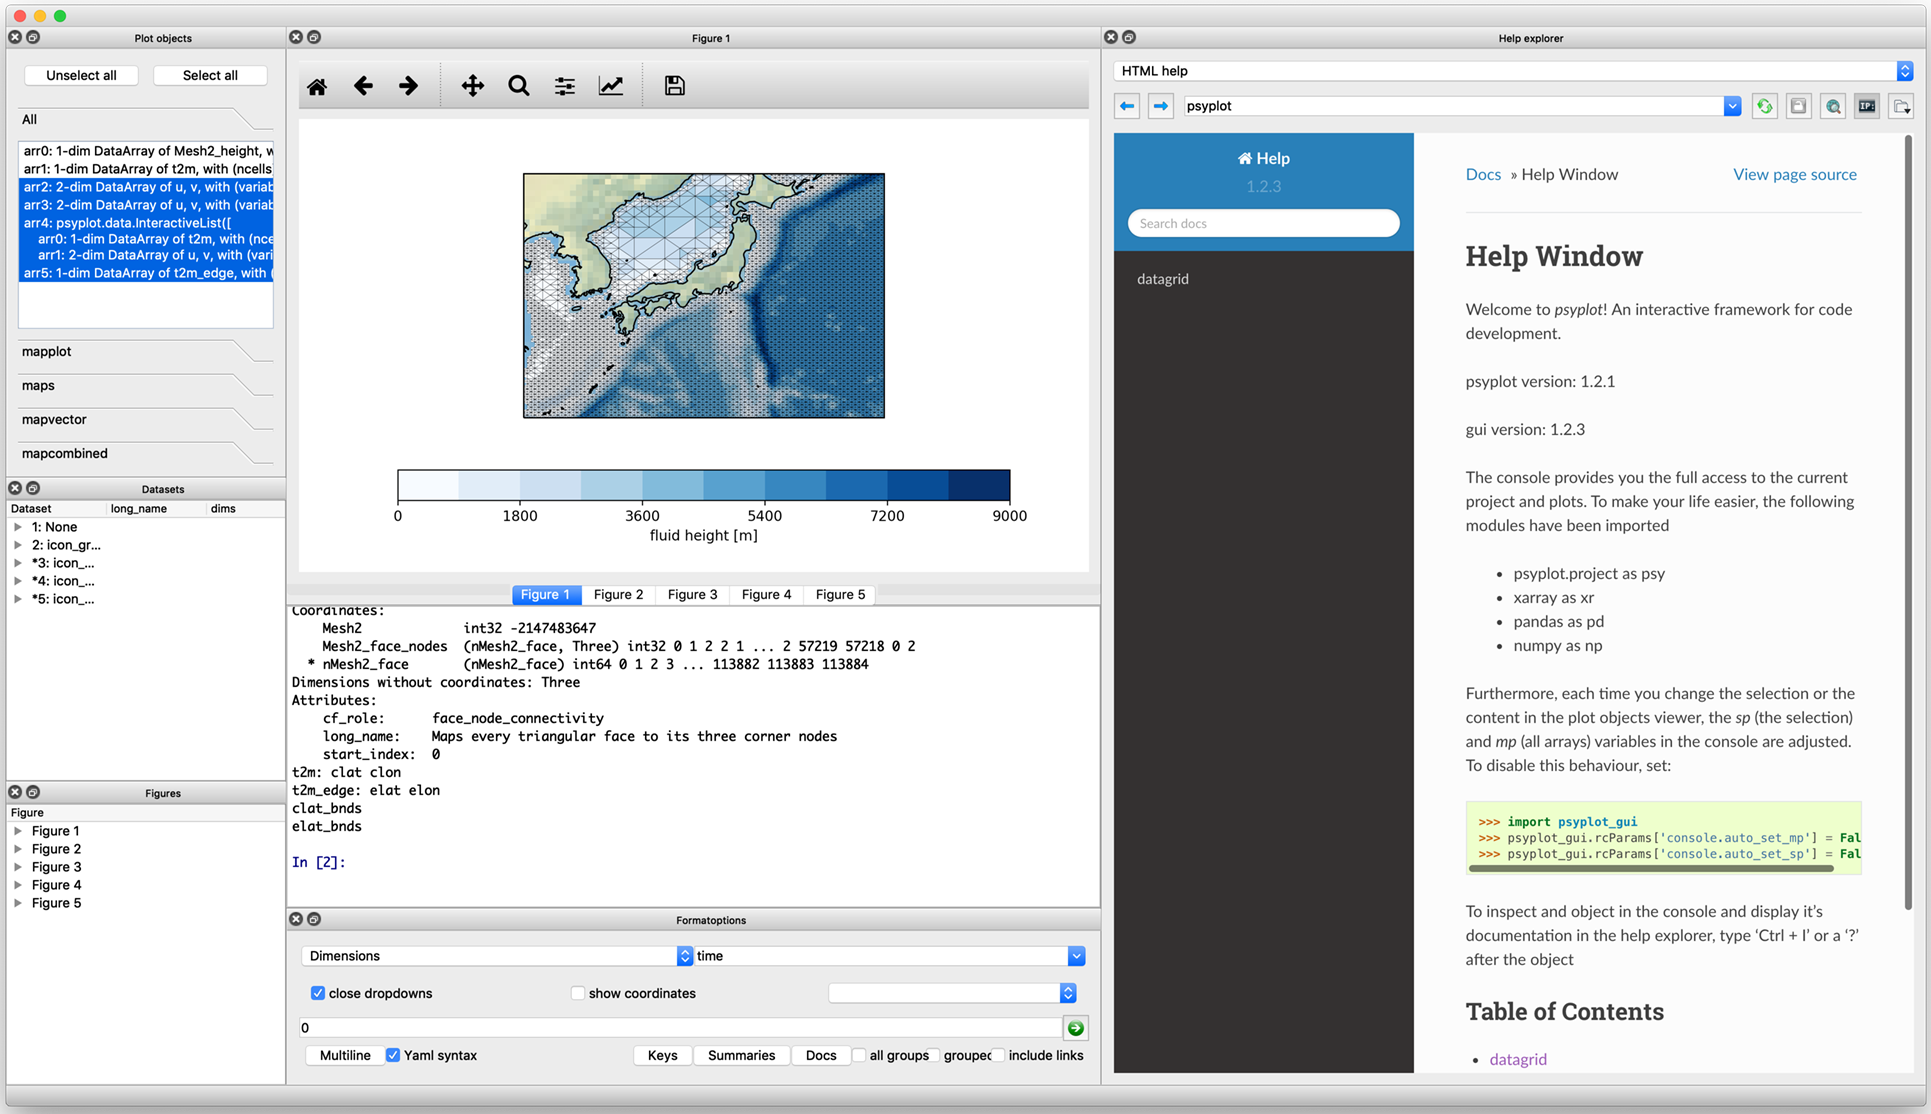
\includegraphics[width=\linewidth]{psyplot-figures/psyplot-gui.png}};
		\node[] (figures) [above=of image, xshift=-0.1\linewidth, yshift=-0.5cm, fill=red!50] {Figures};
		\node (project) [left=of figures, xshift=-0.1\linewidth, fill=red!50] {Project content};
		\node (help) [right=of figures, xshift=0.2\linewidth, fill=red!50] {Help explorer};
		\node (formatoptions) [below=of image, xshift=-0.1\linewidth, yshift=0.5cm, fill=red!50] {Formatoptions};
		\node (console) [above=of formatoptions, yshift=1.5cm, fill=red!50] {Console};
	\end{tikzpicture}
%	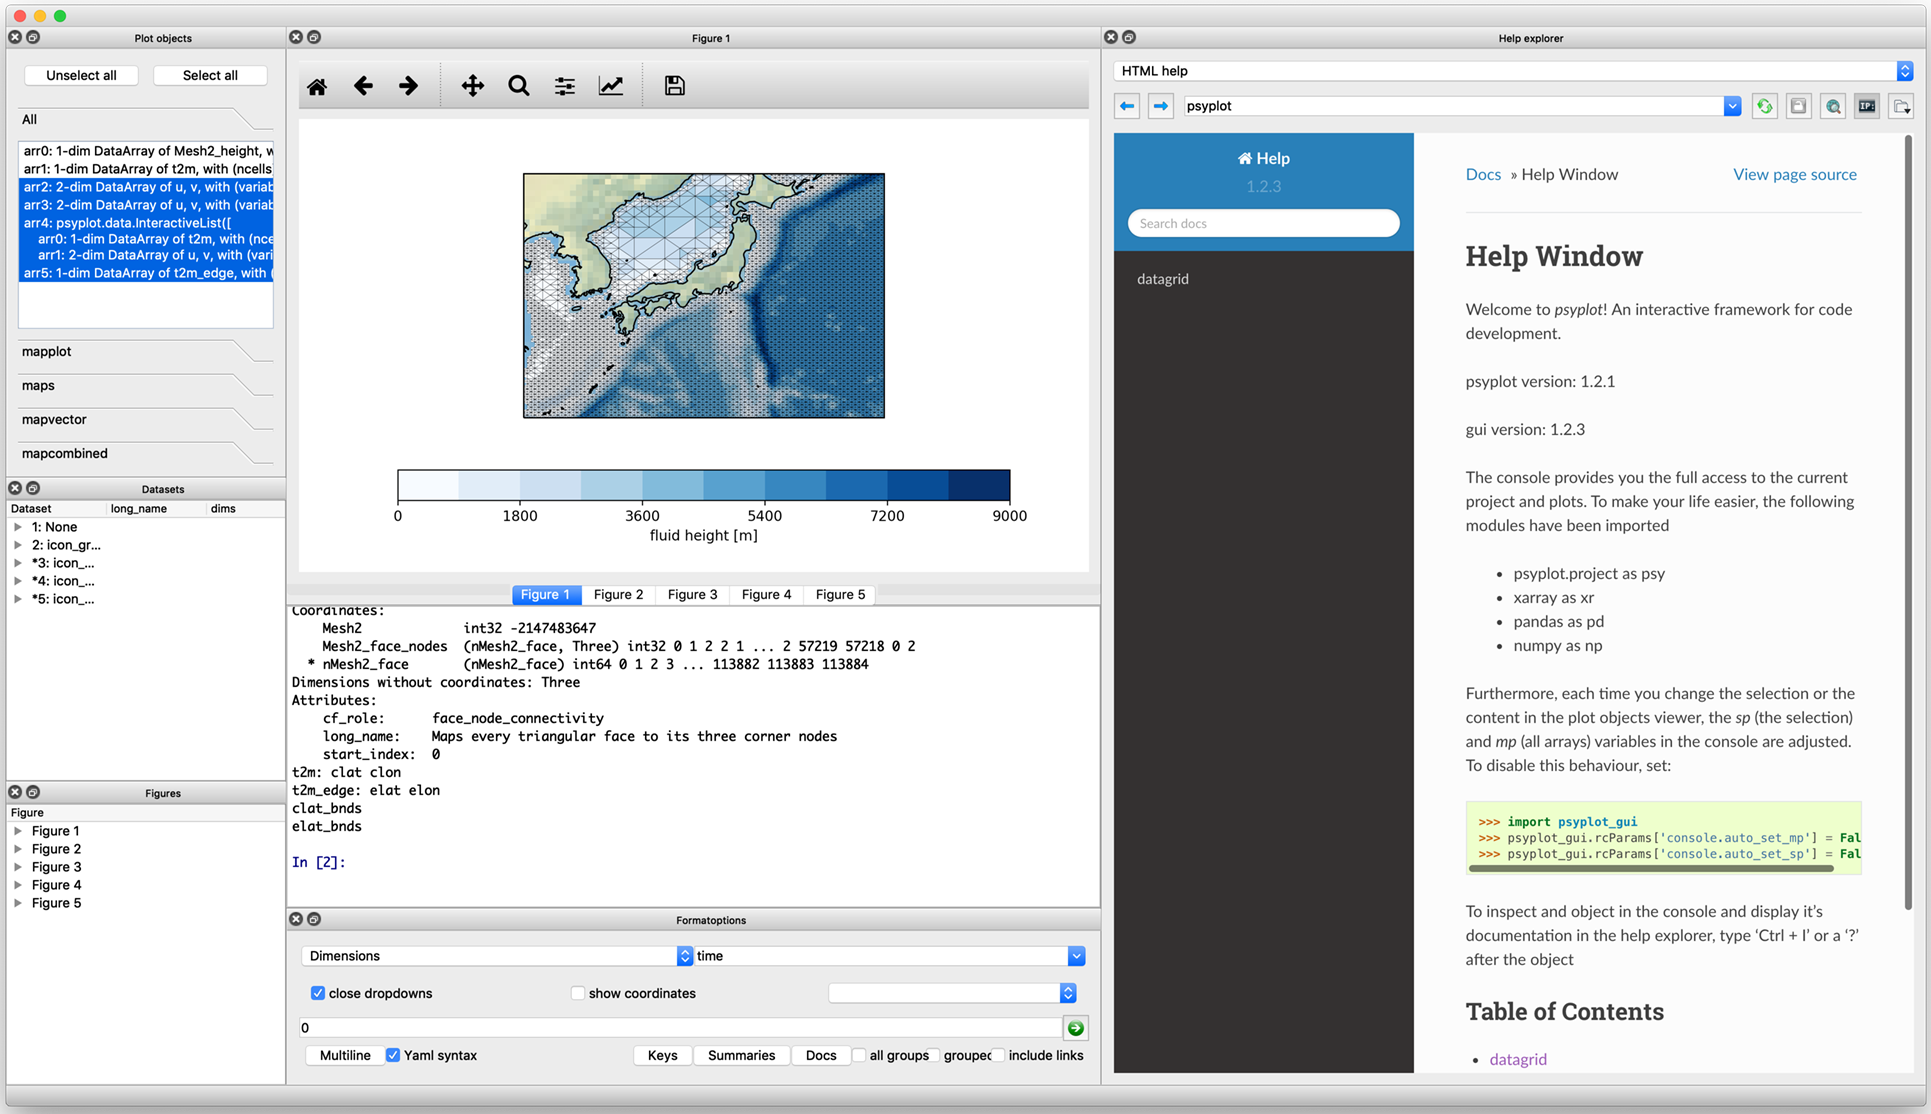
\includegraphics[width=\linewidth]{psyplot-figures/psyplot-gui.png}
	\caption[Screenshot of the psyplot GUI]{Screenshot of the psyplot \gls{gui}. The left part shows the content of the psyplot project, the upper center the plots, and the right part contains the help explorer. Below the plots, there is also the IPython console for the usage from the command line and a widget to update the formatoptions of the current project.}
	\label{fig:psyplot-gui}
\end{figure}

\begin{figure}
	\centering
	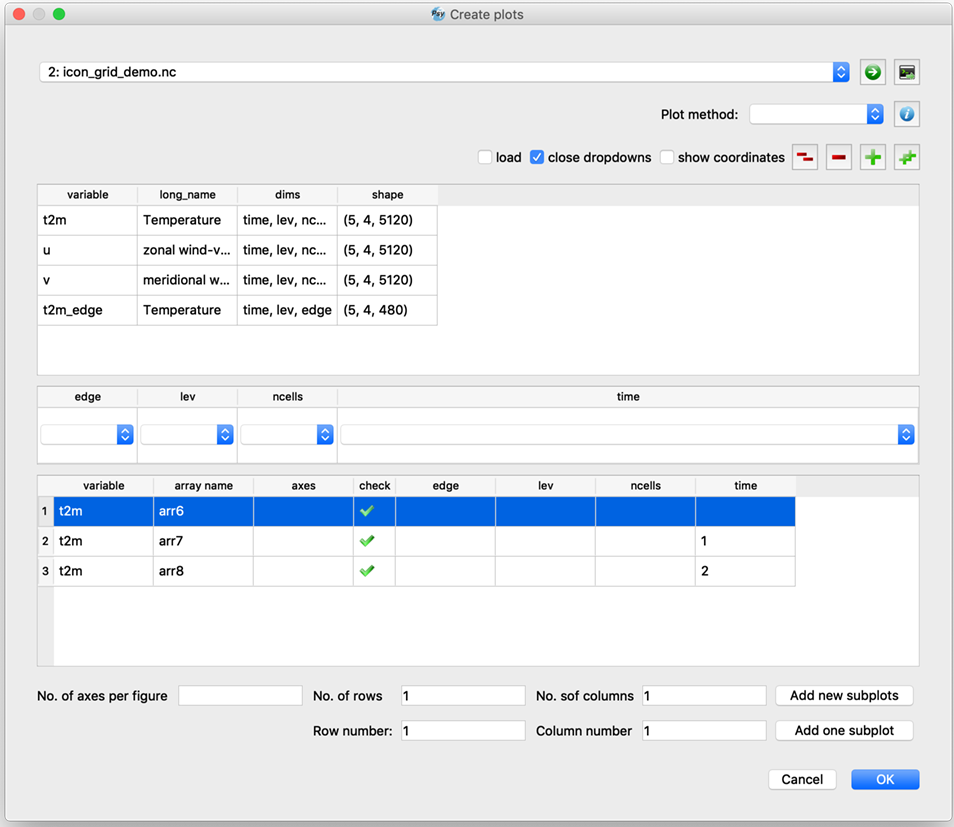
\includegraphics[width=0.7\linewidth]{psyplot-figures/plot-creator.png}
	\caption[psyplot Gui plot creation dialog]{Plot creation dialog to generate new figures from an xarray dataset.}
	\label{fig:psyplot-gui-plot-creator}
\end{figure}

Psyplots objective of providing a platform for flexible and convenient data analysis is complemented through the psyplot\_gui package. This extension to the framwork provides a \gls{gui} for simplified access to the plotting features in psyplot.

A strong focus is, again, the flexibility of the interface. The package is based on the cross-platform library PyQt5\footnote{PyQt5 can be accessed via \url{https://riverbankcomputing.com/software/pyqt/intro}.}, a very flexible and frequently used package for \acrlongpl{gui}. This enables other software to develop additional features for the package (see psy-strat in the previous section \ref{sec:psyplot-plugins} or straditize in chapter \ref{chp:straditize}) and to flexibly change the layout of the application. The \gls{gui} is additionally complemented with an interactive console to enable a fully integrated python environment for data analysis. This enables the user to run every python command and to load additional packages. 

The next paragraphs provide an overview on the various features, that are also displayed in figure \ref{fig:psyplot-gui} and \ref{fig:psyplot-gui-plot-creator}.

\subsubsection{Console}
An in-process IPython console based on the qtconsole package\footnote{\url{https://github.com/jupyter/qtconsole}} that provides the possibility to communicate with the psyplot package via the command line and to load any other module or to run any other script or notebook. The console is fully integrated into the \gls{gui}. A change of the current project through the project content widgets (see below), for instance,  also changes the corresponding python variable in the shell. Additionally, the documentation of every python object in the shell can be viewed in the help explorer of the GUI (see below).

\subsubsection{Help explorer}
\rewrite{Motivated by the Object inspector of the Scientific PYthon Development EnviRonment Spyder, this widget provides a simple online browser and the possibility to show the documentation of Python objects as an html webpage. The help explorer is connected to several widgets of the GUI and especially to the console, to show the documentation of any python object.}

\subsubsection{Plot creator}
\rewrite{A widget to select data from a dataset and visualise it with a plot method of the psyplot package}

\subsubsection{Project content}
\rewrite{Shows the data arrays, the open datasets and the open figures in the current project}

\subsubsection{Figures and plots}
\rewrite{Displays the matplotlib figures based on an own backend}

\subsubsection{Formatoptions}
\rewrite{Can be used to change the formatoptions}

\section{Conclusions}  \label{sec:psyplot-conclusions}
\todo[inline, size=\normalsize]{Further developments with GUI, 3D, shapefiles, other plot methods}

\clearpage

\begin{subappendices}
	\section*{Supplementary material}
	\section{Example call of a plot method}  \label{sec:psyplot-example}
	
	
	\section{psy-simple plot methods}  \label{sec:psy-simple-plotmethods}
	
		\begin{tabular}{l|p{0.25\linewidth}|p{0.25\linewidth}|p{0.25\linewidth}|}
			\toprule
			\textbf{Plot method} & lineplot & barplot & violinplot \\
			\hline
			\textbf{Example} & \missingfigure{lineplot} & \missingfigure{barplot} & \missingfigure{violinplot} \\
			\midrule
			\midrule
			\textbf{Plot method} & \multicolumn{3}{c}{plot2d} \\
			\hline
			\textbf{Grid type} & rectilinear & \multicolumn{2}{c}{unstructured} \\
			\hline
			\textbf{Example} & \missingfigure{simple 2D plot} & \missingfigure{simple unstructured plot} & \missingfigure{simple unstructured plot with varying cell size} \\
			\midrule
			\midrule
			\textbf{Plot method} & \multicolumn{2}{c|}{vector} & combined \\
			\hline
			\textbf{Example} & \missingfigure{quiver} & \missingfigure{streamlines} & \missingfigure{combined} \\
			\midrule
			\midrule
			\textbf{Plot method} & \multicolumn{2}{c|}{density} & fldmean  \\
			\hline
			\textbf{Example} & \missingfigure{density hist} & \missingfigure{density kde} & \missingfigure{fldmean} \\
			\bottomrule
		\end{tabular}
	

	\section{psy-maps plot methods}  \label{sec:psy-maps-plotmethods}
	
		\begin{tabular}{l|p{0.25\linewidth}|p{0.25\linewidth}|p{0.25\linewidth}|}
			\toprule
			\textbf{Plot method} & \multicolumn{3}{c}{mapplot} \\
			\hline
			\textbf{Grid type} & rectilinear & \multicolumn{2}{c}{unstructured} \\
			\hline
			\textbf{Example} & \missingfigure{map 2D plot} & \missingfigure{map unstructured plot} & \missingfigure{map unstructured plot with varying cell size} \\
			\midrule
			\midrule
			\textbf{Plot method} & \multicolumn{2}{c|}{mapvector} & combined \\
			\hline
			\textbf{Example} & \missingfigure{map quiver} & \missingfigure{map streamlines} & \missingfigure{map combined} \\
			\bottomrule
		\end{tabular}
	
	\section{psy-reg plot methods}  \label{sec:psy-reg-plotmethods}
	
		\begin{tabular}{l|p{0.25\linewidth}|p{0.25\linewidth}|}
			\toprule
			\textbf{Plot method} & \multicolumn{2}{c}{linreg} \\
			\hline
			\textbf{Example} & \missingfigure{linreg simple} & \missingfigure{linreg curvy} \\
			\midrule
			\midrule
			\textbf{Plot method} & \multicolumn{2}{c|}{densityreg} \\
			\hline
			\textbf{Example} & \missingfigure{densityreg simple} & \missingfigure{densityreg curvy} \\
			\bottomrule
		\end{tabular}
	
	\section{psy-strat plot methods}  \label{sec:psy-strat-plotmethods}

		\missingfigure{stratigraphic diagram (straditize paper?)}

\end{subappendices}\

\printbibliography[heading=subbibintoc]

\end{refsection}